% Options for packages loaded elsewhere
\PassOptionsToPackage{unicode}{hyperref}
\PassOptionsToPackage{hyphens}{url}
%
\documentclass[
  english,
  ,jou]{apa6}
\usepackage{lmodern}
\usepackage{amssymb,amsmath}
\usepackage{ifxetex,ifluatex}
\ifnum 0\ifxetex 1\fi\ifluatex 1\fi=0 % if pdftex
  \usepackage[T1]{fontenc}
  \usepackage[utf8]{inputenc}
  \usepackage{textcomp} % provide euro and other symbols
\else % if luatex or xetex
  \usepackage{unicode-math}
  \defaultfontfeatures{Scale=MatchLowercase}
  \defaultfontfeatures[\rmfamily]{Ligatures=TeX,Scale=1}
\fi
% Use upquote if available, for straight quotes in verbatim environments
\IfFileExists{upquote.sty}{\usepackage{upquote}}{}
\IfFileExists{microtype.sty}{% use microtype if available
  \usepackage[]{microtype}
  \UseMicrotypeSet[protrusion]{basicmath} % disable protrusion for tt fonts
}{}
\makeatletter
\@ifundefined{KOMAClassName}{% if non-KOMA class
  \IfFileExists{parskip.sty}{%
    \usepackage{parskip}
  }{% else
    \setlength{\parindent}{0pt}
    \setlength{\parskip}{6pt plus 2pt minus 1pt}}
}{% if KOMA class
  \KOMAoptions{parskip=half}}
\makeatother
\usepackage{xcolor}
\IfFileExists{xurl.sty}{\usepackage{xurl}}{} % add URL line breaks if available
\IfFileExists{bookmark.sty}{\usepackage{bookmark}}{\usepackage{hyperref}}
\hypersetup{
  pdftitle={Crossing a River to get some Water? An Empirical Comparison of Classic and Contemporary Approaches to Item Social Desirability Evaluation},
  pdfauthor={John T. Kulas1, Emily J. Johnson2, \& Julia Wefferling1},
  pdflang={en-EN},
  pdfkeywords={Social Desirability, Bias, Item Characteristics},
  hidelinks,
  pdfcreator={LaTeX via pandoc}}
\urlstyle{same} % disable monospaced font for URLs
\usepackage{graphicx,grffile}
\makeatletter
\def\maxwidth{\ifdim\Gin@nat@width>\linewidth\linewidth\else\Gin@nat@width\fi}
\def\maxheight{\ifdim\Gin@nat@height>\textheight\textheight\else\Gin@nat@height\fi}
\makeatother
% Scale images if necessary, so that they will not overflow the page
% margins by default, and it is still possible to overwrite the defaults
% using explicit options in \includegraphics[width, height, ...]{}
\setkeys{Gin}{width=\maxwidth,height=\maxheight,keepaspectratio}
% Set default figure placement to htbp
\makeatletter
\def\fps@figure{htbp}
\makeatother
\setlength{\emergencystretch}{3em} % prevent overfull lines
\providecommand{\tightlist}{%
  \setlength{\itemsep}{0pt}\setlength{\parskip}{0pt}}
\setcounter{secnumdepth}{-\maxdimen} % remove section numbering
% Make \paragraph and \subparagraph free-standing
\ifx\paragraph\undefined\else
  \let\oldparagraph\paragraph
  \renewcommand{\paragraph}[1]{\oldparagraph{#1}\mbox{}}
\fi
\ifx\subparagraph\undefined\else
  \let\oldsubparagraph\subparagraph
  \renewcommand{\subparagraph}[1]{\oldsubparagraph{#1}\mbox{}}
\fi
% Manuscript styling
\usepackage{upgreek}
\captionsetup{font=singlespacing,justification=justified}

% Table formatting
\usepackage{longtable}
\usepackage{lscape}
% \usepackage[counterclockwise]{rotating}   % Landscape page setup for large tables
\usepackage{multirow}		% Table styling
\usepackage{tabularx}		% Control Column width
\usepackage[flushleft]{threeparttable}	% Allows for three part tables with a specified notes section
\usepackage{threeparttablex}            % Lets threeparttable work with longtable

% Create new environments so endfloat can handle them
% \newenvironment{ltable}
%   {\begin{landscape}\begin{center}\begin{threeparttable}}
%   {\end{threeparttable}\end{center}\end{landscape}}
\newenvironment{lltable}{\begin{landscape}\begin{center}\begin{ThreePartTable}}{\end{ThreePartTable}\end{center}\end{landscape}}

% Enables adjusting longtable caption width to table width
% Solution found at http://golatex.de/longtable-mit-caption-so-breit-wie-die-tabelle-t15767.html
\makeatletter
\newcommand\LastLTentrywidth{1em}
\newlength\longtablewidth
\setlength{\longtablewidth}{1in}
\newcommand{\getlongtablewidth}{\begingroup \ifcsname LT@\roman{LT@tables}\endcsname \global\longtablewidth=0pt \renewcommand{\LT@entry}[2]{\global\advance\longtablewidth by ##2\relax\gdef\LastLTentrywidth{##2}}\@nameuse{LT@\roman{LT@tables}} \fi \endgroup}

% \setlength{\parindent}{0.5in}
% \setlength{\parskip}{0pt plus 0pt minus 0pt}

% \usepackage{etoolbox}
\makeatletter
\patchcmd{\HyOrg@maketitle}
  {\section{\normalfont\normalsize\abstractname}}
  {\section*{\normalfont\normalsize\abstractname}}
  {}{\typeout{Failed to patch abstract.}}
\patchcmd{\HyOrg@maketitle}
  {\section{\protect\normalfont{\@title}}}
  {\section*{\protect\normalfont{\@title}}}
  {}{\typeout{Failed to patch title.}}
\makeatother
\shorttitle{ITEM SD RATINGS}
\keywords{Social Desirability, Bias, Item Characteristics}
\usepackage{dblfloatfix}


\usepackage{csquotes}
\usepackage{pdflscape}
\newcommand{\blandscape}{\begin{landscape}}
\newcommand{\elandscape}{\end{landscape}}
\ifxetex
  % Load polyglossia as late as possible: uses bidi with RTL langages (e.g. Hebrew, Arabic)
  \usepackage{polyglossia}
  \setmainlanguage[]{english}
\else
  \usepackage[shorthands=off,main=english]{babel}
\fi

\title{Crossing a River to get some Water? An Empirical Comparison of Classic and Contemporary Approaches to Item Social Desirability Evaluation}
\author{John T. Kulas\textsuperscript{1}, Emily J. Johnson\textsuperscript{2}, \& Julia Wefferling\textsuperscript{1}}
\date{}


\affiliation{\vspace{0.5cm}\textsuperscript{1} Montclair State University\\\textsuperscript{2} St.~Cloud State University}

\abstract{
Traditional approaches to the assessment of socially desirable content within assessment indicators have been implicated as being too simple. Correspondingly, an alternative method (Kuncel \& Tellegen, 2009) has been proposed. The current study examines whether the added complexity of the newer procedure is accompanied by a substantially meaningful additional amount of unique information regarding the socially desirable content of instrument indicators. Findings suggest that the two procedures may benefit from mutual application. Specifically, the more cognitively taxing newer procedure may be best leveraged with indicators first implicated as ``moderate'' via application of the traditional (Edwards, 1953, 1957a) approach. A traditionally simple (Edwards, 1953) and more contemporary complex approach (Kuncel \& Tellegen, 2009) to collect indications of socially desirable content within assessment indicators were empirically compared and contrasted. Results suggest that although the contemporary approach captures some unique information, this is in fact only incrementally informative in predictably particular instances. In other instances, these two approaches convey similar information. These results suggest that the simpler approach should be considered before pursuing the more cognitively-taxing and time-intensive contemporary approach. A more limited application of the contemporary approach should benefit both researchers and item judges.
}



\begin{document}
\maketitle

It may be human nature to lean toward presenting oneself favorably see, for example, Taylor and Brown (1988){]}, however, different contexts are known to prime this tendency. For example, individuals may feel compelled to present themselves in a favorable manner possibly inconsistent with their own true character in situations that call for high-stakes judgements {[}such as a job interview, e.g., (Barrick, Shaffer, \& DeGrassi, 2009; Levashina \& Campion, 2006; Weiss \& Feldman, 2006){]}. These proclivities are generally referred to as acts consistent with a response motive of \emph{social desirability}, and concern individuals' perceptions of what characteristics are generally valued or desired rather than what may be true of the person him or herself (Kuncel \& Tellegen, 2009; Ziegler, 2011).

In psychological testing applications, social desirability refers to the motivation to choose response options that are not necessarily consistent with standing (along the psychological trait), but are rather more socially acceptable (than are alternative responses). When an individual endorses an inventory or assessment item in this manner, they are providing possibly inaccurate information (Fischer \& Fick, 1993), which poses obvious problems for evaluation (for example, failing to identify the better {[}along a focal trait of job relevance{]} applicant out of a pool of honest and socially-desirable prone selection screen respondents).

\#\#The Role of Social Desirability in Psychological Assessment

Two popular contemporary methodologies have been most commonly used to evaluate the impact of social desirability on assessment scores, and both generally support the conclusion that social desirability should not be considered problematic (e.g., it is a ``red herring''; e.g., Ones, Viswesvaran, \& Reiss, 1996). The first popular contemporary methodology involves assessing individual differences in socially desirable response tendencies via questionnaires. For those concerned with response inflation (e.g., selection specialists), individual differences in social desirable tendencies can be leveraged to partial out effects via covariate specification. Common measures used in this application are, for example, the Balanced Inventory of Desirable Responding (BIDR), or the Crowne-Marlowe social desirability scale (e.g., see Li \& Bagger, 2006).

The second set of popular contemporary methodologies employs experimental instructions to \enquote{fake} responses or comparisons of job applicant versus non-applicant respondents (e.g., Birkeland, Manson, Kisamore, Brannick, \& Smith, 2006; Viswesvaran \& Ones, 1999). Patterns of response are then investigated under conditions thought to be susceptible to socially desirable responding (e.g., fake experimental conditions or applicant respondent samples) versus conditions purported to be lacking socially desirable influence (e.g., control or respond honest experimental conditions, and non-applicant respondents).

The meta-analyses of Birkeland et al. (2006), Ones et al. (1996), and Viswesvaran and Ones (1999) summarize findings across studies applying these common approaches. Ones et al. (1996)'s approach investigated individual differences in socially desirable responding (as assessed via individual difference measures such as the BIDR), and used this level of association to construct, for example, semipartial correlations between Big 5 scales and work-relevant criteria (e.g., training performance, counterproductive behaviors, job performance). There was little effect noted of socially desirable response tendencies on criterion-related validities in Ones et al. (1996)'s meta-analysis.

Viswesvaran and Ones (1999) applied a similar meta-analytic lens to experimental investigations involving instructions to \enquote{fake good} or \enquote{fake bad}, finding that Big 5 scales tended to exhibit similar levels of fakability. This study confirmed that respondents can indeed fake (e.g., respond in a socially desirable manner) their responses if instructed to do so. Regarding non-laboratory investigations where context is assumed to prime a socially desirable response set, Birkeland et al. (2006) similarly documented elevated Big 5 scale scores with applicant respondents relative to non-applicant respondents, but also noted that the pattern of elevation differed across the type of position the applicant was seeking. Note here that both traditions are characterized by an individual difference orientation (e.g., it is differences across respondent proclivity to enhance {[}either driven by context or trait{]} within which social desirability is manifest).

Alternative to these two very common approaches to exploring social desirability's role in psychological assessment (particularly work-relevant psychological assessment), some researchers have focused on assessment elements themselves (e.g., the \emph{item}; see, for example, Edwards, 1957a). This seems to be more popular in non-work assessment domains than with the I-O literature (see, for example, Leising, Ostrovski, \& Borkenau, 2012; Leising, Scherbaum, Locke, \& Zimmermann, 2015). Traditionally, this approach has been applied in a fairly straightforward manner, with little deviation from Edwards (1953)\enquote{s initial procedure. Originally, Edwards (1953) solicited judges to rate the content of personality items along a social desirability continuum (wherein, for example, the personality item, \enquote{I hate all people} would likely be deemed less desirable than an item such as, \enquote{I regularly give money to charities in need}). Edwards specifically asked his judges to rate personality items from extremely undesirable to extremely desirable on a 9-point scale (and went on to further demonstrate that the more socially desirable an item is, the more likely someone will endorse having that characteristic; Edwards, 1953, 1957a)\footnote{This is a very interesting finding, and one that has been replicated several times, but the focus of this exploration is fully \emph{procedural}, and pointed directly at the \emph{method} used to collect item social desirability ratings rather than the larger implications of attraction toward the socially desirable.}. Although this approach remained relatively unaffected by change for a half century, Kuncel and Tellegen (2009) revisited the procedure, arguing that traditional measurement approaches such as Edwards} are too simplistic if we aim to truly understand the breadth and assessment implications of item-level desirability.

Although this procedure approach existed relatively unaffected by change for a half century, Kuncel and Tellegen (2009) revisited the procedure, arguing that traditional measurement approaches such as Edwards' are too simplistic if we aim to truly understand the breadth and assessment implications of item-level desirability. Specifically, Kuncel and Tellegen (2009) noted that past measurement of social desirability has largely ignored the potentially differential attraction to particular inventory \emph{response options}, as opposed to (or in addition to), the level of desirability saturation within the item stem itself. This perspective challenges the (previously implicit) assumption that social desirability manifests itself in a linear fashion across response options, whereby \enquote{agreement} with more or less of a characteristic is (at least monotonically) associated with more or less social desirability.

However, as rightly noted by Kuncel and Tellegen (2009), this assumption is not necessarily warranted, as there are identifiable characteristics with a \emph{most} desirable standing location that is not located at either extreme (consider, for example, \enquote{being quiet} - it is likely most socially desirable to be moderate along the range of this characteristic). Consistent with this perspective, Kuncel and Tellegen (2009) proposed that at least four likely functions of item social desirability exist across scaled response options: linear, non-linear, non-linear monotonic, and weakly non-linear monotonic. These functional forms propose that the slope between \enquote{location of response} (e.g., low, moderate, or high on the trait) and \enquote{how desirable the location is} could be linear, plateaued, \enquote{U}-shaped (or invertedly \enquote{U}-shaped), or perhaps even flat in several regions. The authors even suggested that \emph{most} trait items may be best characterized by nonmonotonic or weakly monotonic relationships with social desirability and that a strictly linear relationship would be dependent on highly valued items or strong incentivized contexts (for example, applying for a desired job).

To test their premise, Kuncel and Tellegen (2009) constructed an alternative rating system. This \enquote{new} approach asks individual judges to rate items on how \emph{desirable it would be considered to be} at different levels of the characteristic: extremely high (top 1\%), above average (top 30\%), average, below average (bottom 30\%), or extremely low (bottom 1\%; see Figure 1, which has been reproduced from the original Kuncel and Tellegen (2009) publication). These five categories approximate the common 5-point rating system frequently encountered in Psychological assessment self-reports. Applying this procedure, Kuncel and Tellegen (2009) found support for their premise that not all items demonstrate linear associations with social desirability and that non-monotonic relationships do exist across graded response continua (for example, \enquote{U}-shaped and inverted \enquote{U}-shaped patterns of social desirability across scaled trait levels).

Kuncel and Tellegen (2009)'s second study was designed to place respondents in a real-world approximation. Here participants were asked to act as if though they were in a pre-employment assessment situation and to also explain their rationale when an extreme response was \emph{not} chosen on the assessment. This clever design was intended to provide insight regarding the lack of linear manifestations of socially desirable responding. Kuncel and Tellegen (2009) found that, across administrations, over 61\% of participants did in fact choose the most extreme response options. Some of the participants who opted out of endorsing the extreme responses, however, noted that the extreme response could be seen as worse (i.e., too inaccurate, bragging, too good). Overall, both studies supported their idea that trait characteristics do not necessarily behave linearly as they relate to the concept of \enquote{desirability} and its manifestation across gradated response options.

\begin{figure}
\centering
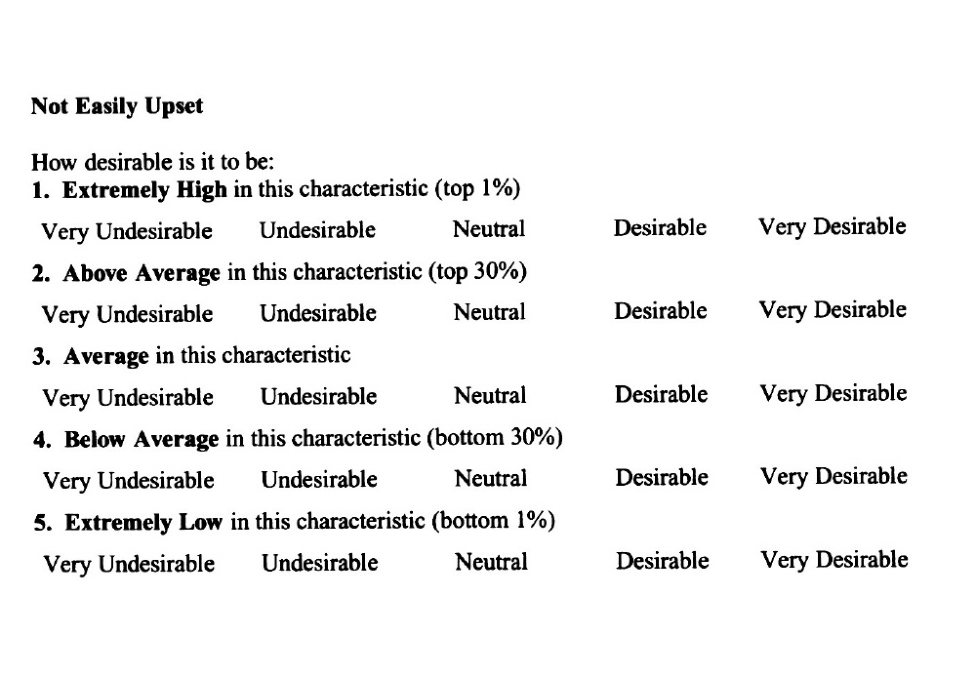
\includegraphics{KuncelTellegen2_files/figure-latex/Figure1-1.pdf}
\caption{\label{fig:Figure1}Kuncel and Tellegen (2009) method for determining socially desirable saturation at the item response level.}
\end{figure}

Although there is both theoretical and empirical support for Kuncel and Tellegen (2009)'s procedure, it also quite substantially more time- and (we propose) effort-intensive than is the traditional item-rating approach (e.g., Edwards, 1957b, p. @edwards\_social\_1957, and @edwards\_relationship\_1953). As technically specified, the \emph{traditional} Edwards procedure requires one evaluation per item, albeit that evaluation is made across nine levels of social desirability. The \emph{contemporary} Kuncel and Tellegen procedure specifies five evaluations across five levels of desirability per item. In addition to the multiplicatively greater \emph{number} of evaluations required in the contemporary approach (requiring a longer time commitment from item judges), we propose that the contemporary approach is also likely more cognitively demanding due to shifting experimental frames (the referent of appraisal is variable across ratings).

Given the greater time and (we argue) resource commitments required of the contemporary approach (relative to the traditional), we aim to gauge to what extent these two approaches in fact capture similar versus unique pieces of information. The goal of the present SIOP investigation is therefore to directly compare these two methodologies with an \enquote{additional information} orientation - that is, is the new approach truly unique, or rather does it at least with some indicators convey somewhat redundant information as the classic, cognitively easier and less time-intensive approach?

\hypertarget{study-1}{%
\section{Study 1}\label{study-1}}

\hypertarget{methods}{%
\section{Methods}\label{methods}}

\hypertarget{participants}{%
\subsection{Participants}\label{participants}}

Seventy-six undergraduate students made ratings of \emph{either} item social desirability (\emph{N} = 14) (Edwards, 1957a), or levels of desirability associated with different trait levels (\emph{N} = 62;(e.g., Kuncel \& Tellegen, 2009)).

\hypertarget{materials}{%
\subsection{Materials}\label{materials}}

The IPIP-NEO is a 300-item personality measure intended to assess the Big Five personality dimensions: Conscientiousness, Agreeableness, Extraversion, Openness to Experience, and Neuroticism (Johnson, 2005). For the purposes of the current investigation, we did not collect typical responses to these 300 indicators, but were rather interested in the nature of the items themselves (or, alternatively, the evaluative content associated with differential standing along the construct implied by the item response options).

\hypertarget{procedure}{%
\subsection{Procedure}\label{procedure}}

Social desirability ratings of the 300 IPIP item stems were made via paper and pencil along a 9-point scale ranging from (-4) Extremely Undesirable to (+4) Extremely Desirable. There were two counterbalanced versions of 150 items each to (attempt to) ward off potential fatigue effects across the rating process. The Kuncel and Tellegen (2009) ratings were performed along one of 10 different counterbalancings - all raters (regardless of task - item stem or response option rating) experienced the same total number of ratings (e.g., the \enquote{Edwards} raters provided one evaluation per 150 items whereas the \enquote{Kuncel \& Tellegen} raters provided five evaluations across 30 items).

In order to model the extremity of function across Kuncel and Tellegen (2009) values, several regressions\footnote{Polynomial regressions were also conducted to capture functional form but are not presented as a central index in this SIOP presentation - these are however available from the authors upon request (this submission was generated via rMarkdown and all data, analyses, and procedural execution are in fact available upon request {[}in the form of an rMarkdown script{]}).} were fit using trait location as a predictor (e.g., Kuncel and Tellegen (2009)'s \enquote{Lower 1\%}, \enquote{Lower 30\%}, \enquote{Median}, \enquote{Upper 30\%}, and \enquote{Upper 1\%} were treated as a scaled continuum) and average desirability rating as the criterion. Slopes were retained for each function, with the expectation that slope magnitude and valence would parallel the classic Edwards ratings.

For this SIOP presentation, we focused on three comparative indices. First, we fit linear regressions to all 300 items' functions, focusing on the slopes, then regressed Edwards' ratings on slope coefficients across items. Secondly, we did a simple frequency accounting for the number of Kuncel and Tellegen (2009) functional types that occured within each categorical strata of Edwards' ratings (e.g., how many \enquote{inverted U-shaped} functions were noted in items characterized as \emph{extremely undesirable}, \emph{undesirable}, \emph{average}, \emph{desirable}, and \emph{extremely desirable}). Thirdly, we visually inspected functional plots within arrays of Edwards' item groupings.\footnote{Note that two of these analyses share some inellegance due to a categorization of Edwards' values (e.g., there are ranges of values within each of these 5 categories; see, for example, Cohen, 1983) - we chose to categorize within crude strata because such oversimplification \emph{does} quite dramatically facilitate the communication of these results.}

\#Results

The plurality of findings do support similar infomration being conveyed through both approaches. Figure 1 captures \emph{some} of this, as functional slopes (even if somewhat nonmonotonic - see, for example, \enquote{Seldom Daydream} in Figure 1) tend to be more extreme with Edwards' highly desirable or undesirable items, and more flat with Edwards' moderate items.\footnote{These items were randomly sampled from within Edwards-rating strata. Visuals of all items' functional forms are available from the authors upon request.} Table 1 presents the frequency with which researcher-implicated functional shapes (linear {[}positive{]}, linear {[}negative{]}, nonmonotonic {[}U{]}, and nonmonotonic {[}inverted U{]}) were noted within \enquote{Edwardian} strata, demonstrating that although the nonmonotonic functions do exist, they are predominantly associated with moderate Edwards items (e.g., yes these functions do occur but perhaps the ambivalence is also associated with aggregate moderation). Figure 2 presents the relationship between: 1) the functional slope relating an item response's rated level of desirability and the \enquote{location} of the rating, and 2) Edwards' item stem rating (on the y-axis). This strong relationship (\emph{R\^{}2} = .67, \emph{p} \textless{} .05) suggests some level of similarity across procedures.

\hypertarget{study-two}{%
\section{Study Two}\label{study-two}}

One of our observations across the two item rating procedures has been that the Kuncel and Tellegen (2009) approach appears to be more cognitively taxing for \enquote{raters} than does the Edwards (1953). Study Two therefore collected ratings via computer, with response latencies recorded as well as direct self-reported estimates of difficulty. The same indicators were retained for Study Two.

\hypertarget{procedure-1}{%
\subsection{Procedure}\label{procedure-1}}

The Study One items were administered via Qualtrics (2014). Participants were administered directions for each condition: 1) Edwards rating, 2) Kuncel \& Tellegen rating, and 3) modified Kuncel \& Tellegen rating. This third condition was included as a possible compromise to the \emph{anticipated} cognitive difficulty associated with the Kuncel \& Tellegen procedure. Here, we ask participants to focus on only one of the Kuncel \& Tellegen \enquote{levels} (e.g., across items, the rating category is held constant). We coded items for length and presence of a \enquote{negative} qualifier (e.g., I would never lie). Anecdotally, the presence of a negative element within an item stem contributed to difficulty for raters.

In addition to actual ratings, we also recorded latencies, direct assessments of difficulty.

Table to add: ICC's for each condition

Focus on response latencies (Edwards ratings vs.~Kuncel \& Tellegen vs.~revised Kuncel \& Tellegen (split by rated category). Indices here are: 1) response latencies, 2) inter-rater agreement/reliability\footnote{NOTE TO SELVES - WHEN WE DO THE SECOND PART (RESPONSE LATENCIES), MAKE SURE TO CODE NEGATIVELY-WORDED STEMS (THESE SEEM ESPECIALLY DIFFICULT TO RATE USING THE KUNCEL \& TELLEGEN PROCEDURE)}

\hypertarget{results}{%
\section{Results}\label{results}}

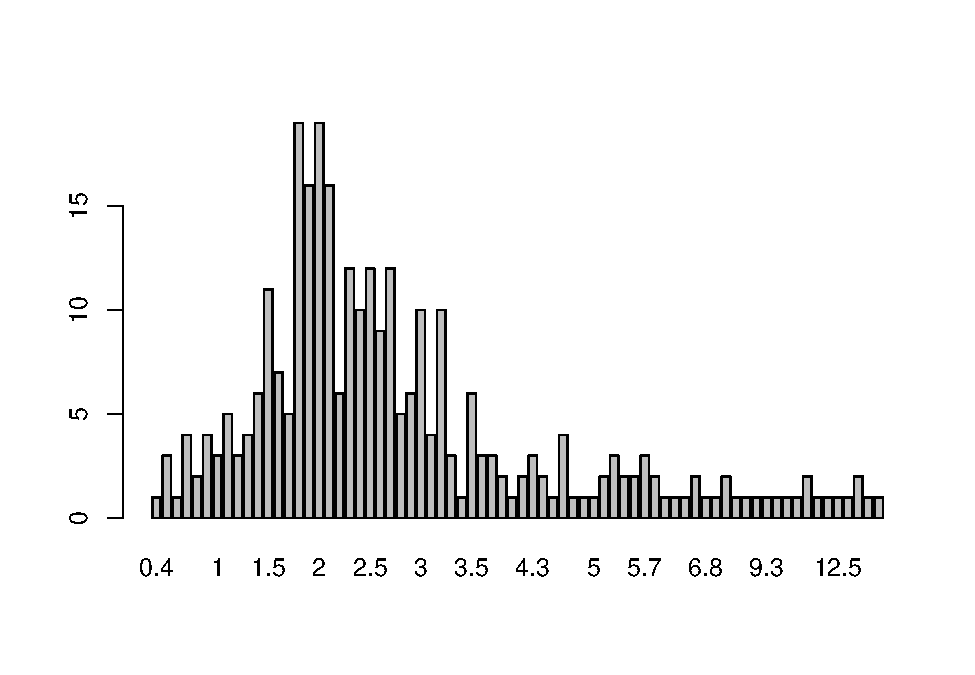
\includegraphics{KuncelTellegen2_files/figure-latex/getQualtrics-1.pdf}

\begin{verbatim}
## latr 
##       Frequency  Percent Valid Percent
## 0.4           1   0.3322        0.3344
## 0.5           3   0.9967        1.0033
## 0.6           1   0.3322        0.3344
## 0.7           4   1.3289        1.3378
## 0.8           2   0.6645        0.6689
## 0.9           4   1.3289        1.3378
## 1             3   0.9967        1.0033
## 1.1           5   1.6611        1.6722
## 1.2           3   0.9967        1.0033
## 1.3           4   1.3289        1.3378
## 1.4           6   1.9934        2.0067
## 1.5          11   3.6545        3.6789
## 1.6           7   2.3256        2.3411
## 1.7           5   1.6611        1.6722
## 1.8          19   6.3123        6.3545
## 1.9          16   5.3156        5.3512
## 2            19   6.3123        6.3545
## 2.1          16   5.3156        5.3512
## 2.2           6   1.9934        2.0067
## 2.3          12   3.9867        4.0134
## 2.4          10   3.3223        3.3445
## 2.5          12   3.9867        4.0134
## 2.6           9   2.9900        3.0100
## 2.7          12   3.9867        4.0134
## 2.8           5   1.6611        1.6722
## 2.9           6   1.9934        2.0067
## 3            10   3.3223        3.3445
## 3.1           4   1.3289        1.3378
## 3.2          10   3.3223        3.3445
## 3.3           3   0.9967        1.0033
## 3.4           1   0.3322        0.3344
## 3.5           6   1.9934        2.0067
## 3.7           3   0.9967        1.0033
## 3.8           3   0.9967        1.0033
## 4             2   0.6645        0.6689
## 4.1           1   0.3322        0.3344
## 4.2           2   0.6645        0.6689
## 4.3           3   0.9967        1.0033
## 4.4           2   0.6645        0.6689
## 4.5           1   0.3322        0.3344
## 4.6           4   1.3289        1.3378
## 4.8           1   0.3322        0.3344
## 4.9           1   0.3322        0.3344
## 5             1   0.3322        0.3344
## 5.1           2   0.6645        0.6689
## 5.2           3   0.9967        1.0033
## 5.5           2   0.6645        0.6689
## 5.6           2   0.6645        0.6689
## 5.7           3   0.9967        1.0033
## 5.8           2   0.6645        0.6689
## 5.9           1   0.3322        0.3344
## 6             1   0.3322        0.3344
## 6.4           1   0.3322        0.3344
## 6.5           2   0.6645        0.6689
## 6.8           1   0.3322        0.3344
## 6.9           1   0.3322        0.3344
## 7.1           2   0.6645        0.6689
## 8.1           1   0.3322        0.3344
## 8.3           1   0.3322        0.3344
## 8.4           1   0.3322        0.3344
## 9.3           1   0.3322        0.3344
## 9.5           1   0.3322        0.3344
## 9.6           1   0.3322        0.3344
## 9.8           1   0.3322        0.3344
## 9.9           2   0.6645        0.6689
## 10.6          1   0.3322        0.3344
## 12.1          1   0.3322        0.3344
## 12.5          1   0.3322        0.3344
## 12.7          1   0.3322        0.3344
## 13            2   0.6645        0.6689
## 13.2          1   0.3322        0.3344
## 25.8          1   0.3322        0.3344
## NA's          2   0.6645              
## Total       301 100.0000      100.0000
\end{verbatim}

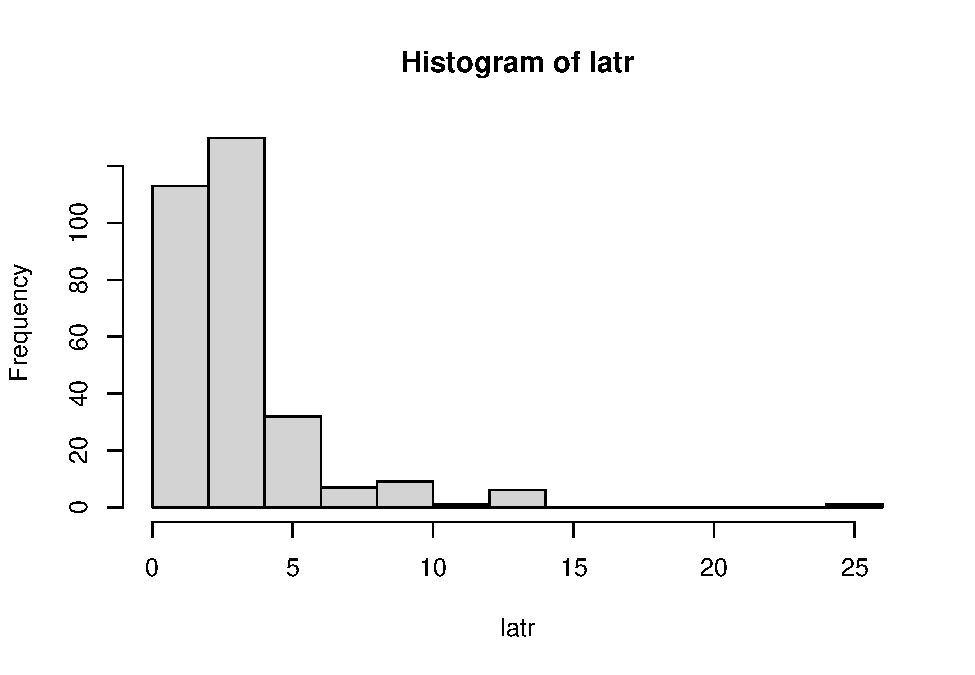
\includegraphics{KuncelTellegen2_files/figure-latex/getQualtrics-2.pdf} 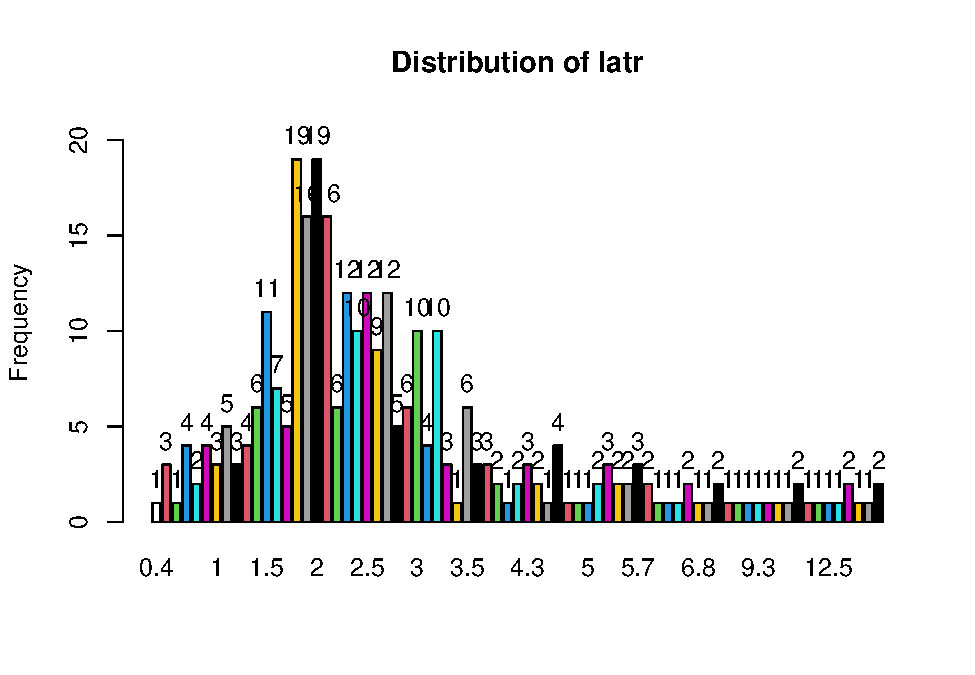
\includegraphics{KuncelTellegen2_files/figure-latex/getQualtrics-3.pdf}

\begin{verbatim}
## latr : 
##         Frequency   %(NA+)   %(NA-)
## 0.4             1      0.3      0.3
## 0.5             3      1.0      1.0
## 0.6             1      0.3      0.3
## 0.7             4      1.3      1.3
## 0.8             2      0.7      0.7
## 0.9             4      1.3      1.3
## 1               3      1.0      1.0
## 1.1             5      1.7      1.7
## 1.2             3      1.0      1.0
## 1.3             4      1.3      1.3
## 1.4             6      2.0      2.0
## 1.5            11      3.7      3.7
## 1.6             7      2.3      2.3
## 1.7             5      1.7      1.7
## 1.8            19      6.3      6.4
## 1.9            16      5.3      5.4
## 2              19      6.3      6.4
## 2.1            16      5.3      5.4
## 2.2             6      2.0      2.0
## 2.3            12      4.0      4.0
## 2.4            10      3.3      3.3
## 2.5            12      4.0      4.0
## 2.6             9      3.0      3.0
## 2.7            12      4.0      4.0
## 2.8             5      1.7      1.7
## 2.9             6      2.0      2.0
## 3              10      3.3      3.3
## 3.1             4      1.3      1.3
## 3.2            10      3.3      3.3
## 3.3             3      1.0      1.0
## 3.4             1      0.3      0.3
## 3.5             6      2.0      2.0
## 3.7             3      1.0      1.0
## 3.8             3      1.0      1.0
## 4               2      0.7      0.7
## 4.1             1      0.3      0.3
## 4.2             2      0.7      0.7
## 4.3             3      1.0      1.0
## 4.4             2      0.7      0.7
## 4.5             1      0.3      0.3
## 4.6             4      1.3      1.3
## 4.8             1      0.3      0.3
## 4.9             1      0.3      0.3
## 5               1      0.3      0.3
## 5.1             2      0.7      0.7
## 5.2             3      1.0      1.0
## 5.5             2      0.7      0.7
## 5.6             2      0.7      0.7
## 5.7             3      1.0      1.0
## 5.8             2      0.7      0.7
## 5.9             1      0.3      0.3
## 6               1      0.3      0.3
## 6.4             1      0.3      0.3
## 6.5             2      0.7      0.7
## 6.8             1      0.3      0.3
## 6.9             1      0.3      0.3
## 7.1             2      0.7      0.7
## 8.1             1      0.3      0.3
## 8.3             1      0.3      0.3
## 8.4             1      0.3      0.3
## 9.3             1      0.3      0.3
## 9.5             1      0.3      0.3
## 9.6             1      0.3      0.3
## 9.8             1      0.3      0.3
## 9.9             2      0.7      0.7
## 10.6            1      0.3      0.3
## 12.1            1      0.3      0.3
## 12.5            1      0.3      0.3
## 12.7            1      0.3      0.3
## 13              2      0.7      0.7
## 13.2            1      0.3      0.3
## 25.8            1      0.3      0.3
## <NA>            2      0.7      0.0
##   Total       301    100.0    100.0
\end{verbatim}

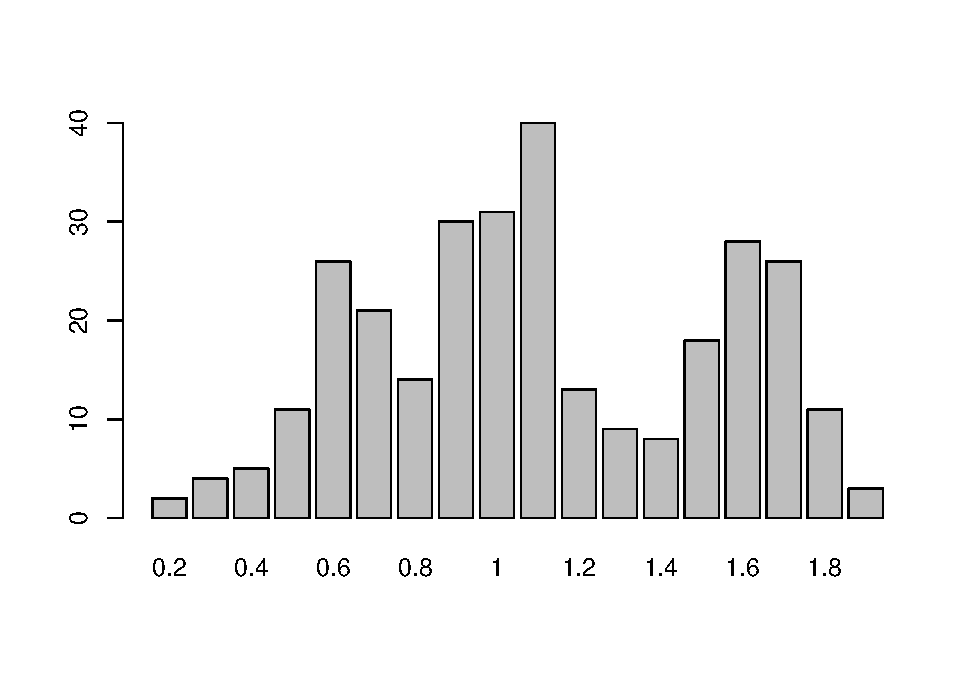
\includegraphics{KuncelTellegen2_files/figure-latex/getQualtrics-4.pdf}

\begin{verbatim}
## latscorer 
##       Frequency  Percent
## 0.2           2   0.6667
## 0.3           4   1.3333
## 0.4           5   1.6667
## 0.5          11   3.6667
## 0.6          26   8.6667
## 0.7          21   7.0000
## 0.8          14   4.6667
## 0.9          30  10.0000
## 1            31  10.3333
## 1.1          40  13.3333
## 1.2          13   4.3333
## 1.3           9   3.0000
## 1.4           8   2.6667
## 1.5          18   6.0000
## 1.6          28   9.3333
## 1.7          26   8.6667
## 1.8          11   3.6667
## 1.9           3   1.0000
## Total       300 100.0000
\end{verbatim}

\hypertarget{discussion}{%
\section{Discussion}\label{discussion}}

Certainly the Kuncel and Tellegen (2009) procedure conveys information not contained in the classic Edwards (1957a) approach. The purpose of this investigation, however, was to document overlap between the two procedures. Clearly nonmonotonic functions do exist for some indicators across scaled \enquote{trait levels}. However, the vast majority of such circumstances are located within what the Edwards (1957a) procedure labels as \enquote{moderately desirable}. There is certainly additional information contained within these items, but the current investigation suggests that perhaps the more cognitively taxing and time-intensive procedure be retained for only those items first identified by the cognitively-easier and less time consuming Edwards (1957a) method as \enquote{moderately desirable}.

\hypertarget{references}{%
\section{References}\label{references}}

\begin{figure}
\centering
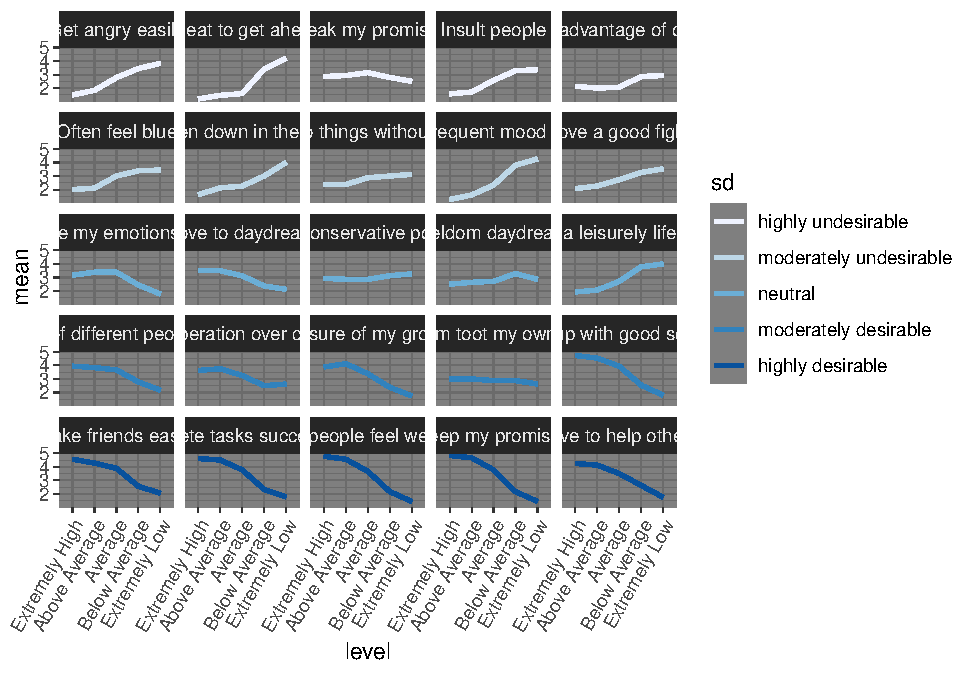
\includegraphics{KuncelTellegen2_files/figure-latex/Figure2-1.pdf}
\caption{\label{fig:Figure2}Kuncel \& Tellegen (2009) patterns across Edwards (1953) scale values.}
\end{figure}

\begin{figure}
\centering
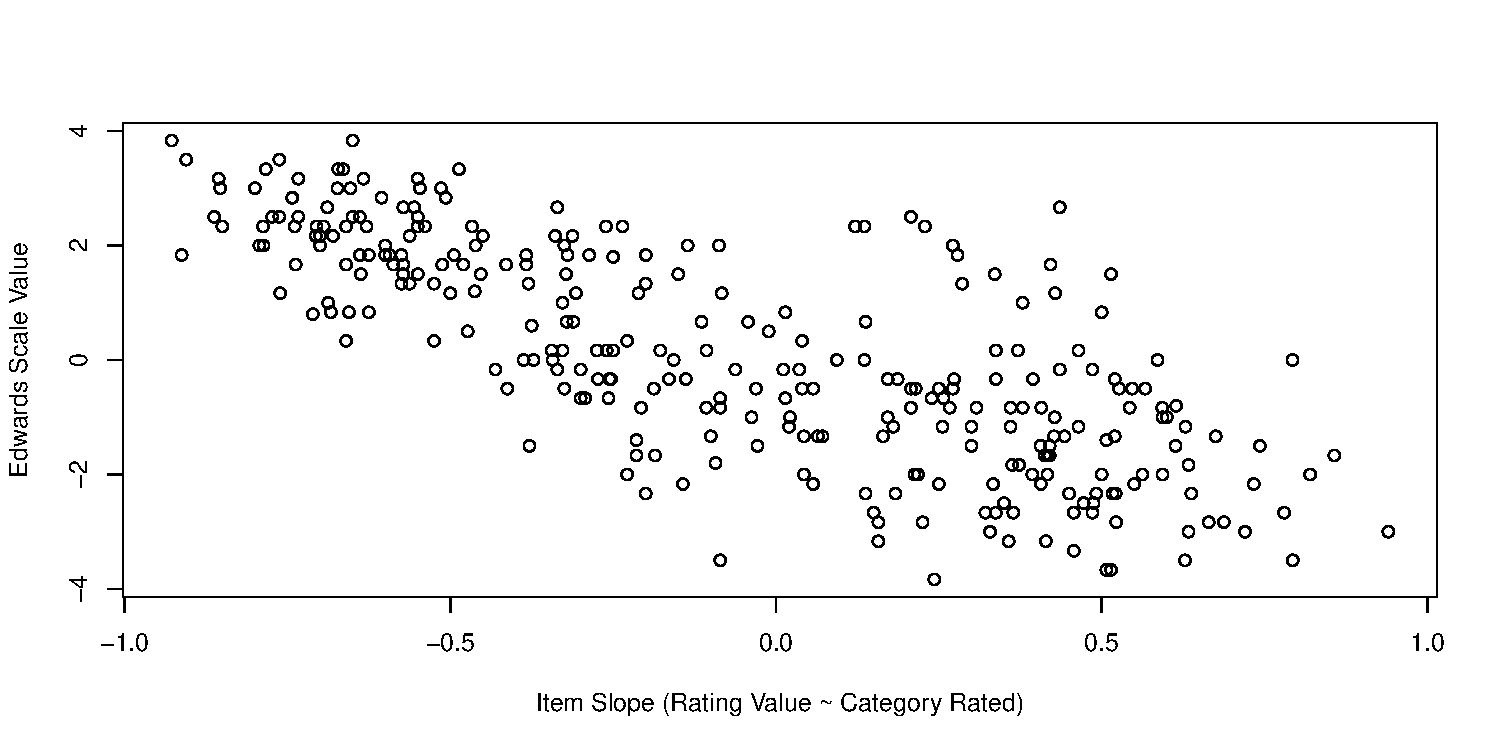
\includegraphics{KuncelTellegen2_files/figure-latex/Figure3-1.pdf}
\caption{\label{fig:Figure3}Response Category and Mean Rating slope across Edwards' scale values (individual scatterpoints represent items).}
\end{figure}

The intercept was -3.08 \textless- just testing.

\begingroup
\setlength{\parindent}{-0.5in}
\setlength{\leftskip}{0.5in}

\hypertarget{refs}{}
\leavevmode\hypertarget{ref-barrick_what_2009}{}%
Barrick, M. R., Shaffer, J. A., \& DeGrassi, S. W. (2009). What you see may not be what you get: Relationships among self-presentation tactics and ratings of interview and job performance. \emph{Journal of Applied Psychology}, \emph{94}(6), 1394.

\leavevmode\hypertarget{ref-birkeland_meta-analytic_2006}{}%
Birkeland, S. A., Manson, T. M., Kisamore, J. L., Brannick, M. T., \& Smith, M. A. (2006). A meta-analytic investigation of job applicant faking on personality measures. \emph{International Journal of Selection and Assessment}, \emph{14}(4), 317--335.

\leavevmode\hypertarget{ref-cohen_cost_1983}{}%
Cohen, J. (1983). The cost of dichotomization. \emph{Applied Psychological Measurement}, \emph{7}(3), 249--253.

\leavevmode\hypertarget{ref-edwards_relationship_1953}{}%
Edwards, A. L. (1953). The relationship between the judged desirability of a trait and the probability that the trait will be endorsed. \emph{Journal of Applied Psychology}, \emph{37}(2), 90.

\leavevmode\hypertarget{ref-edwards_social_1957}{}%
Edwards, A. L. (1957a). Social desirability and probability of endorsement of items in the interpersonal check list. \emph{The Journal of Abnormal and Social Psychology}, \emph{55}(3), 394.

\leavevmode\hypertarget{ref-edwards_social_1957a}{}%
Edwards, A. L. (1957b). \emph{The social desirability variable in personality assessment and research.} New York: Dryden.

\leavevmode\hypertarget{ref-fischer_measuring_1993}{}%
Fischer, D. G., \& Fick, C. (1993). Measuring social desirability: Short forms of the marlowe-crowne social desirability scale. \emph{Educational and Psychological Measurement}, \emph{53}(2), 417--424.

\leavevmode\hypertarget{ref-kuncel_conceptual_2009}{}%
Kuncel, N. R., \& Tellegen, A. (2009). A conceptual and empirical reexamination of the measurement of the social desirability of items: Implications for detecting desirable response style and scale development. \emph{Personnel Psychology}, \emph{62}(2), 201--228.

\leavevmode\hypertarget{ref-leising_vocabulary_2012}{}%
Leising, D., Ostrovski, O., \& Borkenau, P. (2012). Vocabulary for describing disliked persons is more differentiated than vocabulary for describing liked persons. \emph{Journal of Research in Personality}, \emph{46}(4), 393--396.

\leavevmode\hypertarget{ref-leising_model_2015}{}%
Leising, D., Scherbaum, S., Locke, K. D., \& Zimmermann, J. (2015). A model of ``substance'' and ``evaluation'' in person judgments. \emph{Journal of Research in Personality}, \emph{57}(1), 61--71.

\leavevmode\hypertarget{ref-levashina_model_2006}{}%
Levashina, J., \& Campion, M. A. (2006). A model of faking likelihood in the employment interview. \emph{International Journal of Selection and Assessment}, \emph{14}(4), 299--316.

\leavevmode\hypertarget{ref-li_using_2006}{}%
Li, A., \& Bagger, J. (2006). Using the BIDR to distinguish the effects of impression management and self-deception on the criterion validity of personality measures: A meta-analysis. \emph{International Journal of Selection and Assessment}, \emph{14}(2), 131--141.

\leavevmode\hypertarget{ref-ones_role_1996}{}%
Ones, D. S., Viswesvaran, C., \& Reiss, A. D. (1996). Role of social desirability in personality testing for personnel selection: The red herring. \emph{Journal of Applied Psychology}, \emph{81}(6), 660.

\leavevmode\hypertarget{ref-qualtrics_qualtrics_2014}{}%
Qualtrics, L. L. C. (2014). Qualtrics {[}software{]}. \emph{Utah, USA: Qualtrics}.

\leavevmode\hypertarget{ref-taylor_illusion_1988}{}%
Taylor, S. E., \& Brown, J. D. (1988). Illusion and well-being: A social psychological perspective on mental health. \emph{Psychological Bulletin}, \emph{103}(2), 193.

\leavevmode\hypertarget{ref-viswesvaran_meta-analyses_1999}{}%
Viswesvaran, C., \& Ones, D. S. (1999). Meta-analyses of fakability estimates: Implications for personality measurement. \emph{Educational and Psychological Measurement}, \emph{59}(2), 197--210.

\leavevmode\hypertarget{ref-weiss_looking_2006}{}%
Weiss, B., \& Feldman, R. S. (2006). Looking good and lying to do it: Deception as an impression management strategy in job interviews. \emph{Journal of Applied Social Psychology}, \emph{36}(4), 1070--1086.

\leavevmode\hypertarget{ref-ziegler_applicant_2011}{}%
Ziegler, M. (2011). Applicant faking: A look into the black box. \emph{The Industrial and Organizational Psychologist}, \emph{49}(1), 29--36.

\endgroup


\end{document}
